\documentclass[12pt]{article}
\usepackage{graphicx} % Required for inserting images
\usepackage{amsmath}
\usepackage{newtxtext,newtxmath} % Times New Roman font
\usepackage[a4paper, margin=1in]{geometry} % Standard margins
\usepackage{ragged2e} % For text justification
\usepackage{titlesec} % For title formatting
\usepackage{setspace} % Line spacing
\usepackage{array} % Table alignment
\usepackage{graphicx}

\title{\textbf{EENG 482: Signals and Systems}\\ CAT II and Exam}
\date{9th April 2025}
\author{David Muigai}



\begin{document}
\maketitle	
\noindent \textbf{Instructions:} Answer \textbf{All} Questions.
    
    
    \section*{Question 1}
    
    \noindent \textbf{Differentiate between Linear Time Variant (LTV) and Linear Time Invariant (LTI) systems.} \textbf{(2 marks)}
    
    \begin{itemize}
    	\item \textbf{LTI System:} A system is said to be Linear Time Invariant if its behavior and characteristics do not change over time. The output for a given input remains the same, even if the input is shifted in time.
    	
    	\item \textbf{LTV System:} A system is Linear Time Variant if its behavior changes with time. This means the output for a given input may vary if the input is applied at different times.
    \end{itemize}
    
    \section*{Question 2}
    
    \noindent \textbf{Explain what is meant by an invertible system, and using the Z-transform, show that the system described by:}
    
    \[
    y(n) = \sum_{k=-\infty}^{n} x(k)
    \]
    
    \noindent \textbf{is invertible.} \textbf{(3 marks)}
    
    \bigskip
    
    \noindent An \textbf{invertible system} is one in which the original input can be uniquely recovered from the output. That means there exists an inverse system such that when the output is passed through it, the original input is retrieved.
    
    \bigskip
    
    \noindent To verify invertibility, observe that:
    
    \[
    x(n) = y(n) - y(n - 1)
    \]
    
    \noindent Now, taking the Z-transform on both sides:
    
    \[
    X(z) = Y(z) - z^{-1} Y(z) = Y(z)(1 - z^{-1})
    \]
    
    \noindent Therefore:
    
    \[
    H(z) = \frac{Y(z)}{X(z)} = \frac{1}{1 - z^{-1}}
    \]
    
    \noindent The system function \( H(z) \) represents a simple first-order system.
    
    \bigskip
    
    \noindent Now, let's analyze the invertibility:
    
    \[
    H^{-1}(z) = 1 - z^{-1}
    \]
    
    \noindent The inverse system function \( H^{-1}(z) \) is well-defined, indicating that it is possible to uniquely recover the input signal from the output signal.
    
    \bigskip
    
    \noindent Therefore, based on the Z-transform analysis, we can conclude that the system
    
    \[
    y(n) = \sum_{k=-\infty}^{n} x(k)
    \]
    
    \noindent is \textbf{invertible}.
    
    
    
    
    
    
    \section*{Question 3}
    
    Consider a sinusoidal signal:  
    \[
    x(t) = 6 \cos(1000\pi t + 0.2\pi)
    \]  
    which is sampled at a frequency \( F_s = 3 \, \text{kHz} \).
    
    \begin{enumerate}
    	\item[(i)] Determine the expression for the sampled sequence \( x[n] = x(nT_s) \) and determine its Discrete Time Fourier Transform \( X(\omega) = \text{DTFT}\{x[n]\} \).
    	\item[(ii)] Determine \( X(F) = \text{FT}\{x(t)\} \).
    	\item[(iii)] Recompute \( X(\omega) \) from \( X(F) \) and verify that you obtain the same expression as in part (i). \textbf{(8 marks)}
    \end{enumerate}
    
    \subsection*{Solution}
    
    \subsection*{(i) Sampled Signal and DTFT}
    
    Sampling with \( T_s = \frac{1}{F_s} = \frac{1}{3000} \), we have:
    \[
    x[n] = x(nT_s) = 6 \cos(1000\pi n T_s + 0.2\pi) = 6 \cos\left(\frac{\pi}{3} n + 0.2\pi\right)
    \]
    
    Using Euler’s formula:
    \[
    x[n] = 3 e^{j0.2\pi} e^{j\frac{\pi}{3} n} + 3 e^{-j0.2\pi} e^{-j\frac{\pi}{3} n}
    \]
    
    Taking the DTFT:
    \[
    X(\omega) = \text{DTFT}\{x[n]\} = 6\pi e^{j0.2\pi} \delta\left(\omega - \frac{\pi}{3}\right) + 6\pi e^{-j0.2\pi} \delta\left(\omega + \frac{\pi}{3}\right)
    \]
    
    \subsection*{(ii) Continuous-Time Fourier Transform}
    
    Given:
    \[
    x(t) = 6 \cos(1000\pi t + 0.2\pi)
    \]
    
    We rewrite it using Euler's formula:
    \[
    x(t) = 3 e^{j(1000\pi t + 0.2\pi)} + 3 e^{-j(1000\pi t + 0.2\pi)}
    \]
    
    Recall that:
    \[
    \mathcal{F}\{e^{j2\pi F_0 t}\} = \delta(F - F_0)
    \]
    
    Since \( 1000\pi = 2\pi \cdot 500 \), the frequencies are \( \pm500 \, \text{Hz} \). Therefore:
    \[
    X(F) = 3 e^{j0.2\pi} \delta(F - 500) + 3 e^{-j0.2\pi} \delta(F + 500)
    \]
    
    \subsection*{(iii) Recomputing \( X(\omega) \) from \( X(F) \)}
    
    The relation between DTFT and FT is:
    \[
    X(\omega) = F_s \cdot X(F) \bigg|_{F = \frac{\omega F_s}{2\pi}} = 3000 \cdot X\left(\frac{3000 \omega}{2\pi}\right)
    \]
    
    Substituting \( X(F) \) from part (ii):
    \[
    X(\omega) = 3000 \left[3 e^{j0.2\pi} \delta\left(\frac{3000 \omega}{2\pi} - 500\right) + 3 e^{-j0.2\pi} \delta\left(\frac{3000 \omega}{2\pi} + 500\right)\right]
    \]
    
    Using the scaling property of the delta function:
    \[
    \delta\left(a\omega\right) = \frac{1}{|a|} \delta(\omega)
    \]
    
    We get:
    \[
    X(\omega) = 6\pi e^{j0.2\pi} \delta\left(\omega - \frac{\pi}{3}\right) + 6\pi e^{-j0.2\pi} \delta\left(\omega + \frac{\pi}{3}\right)
    \]
    
    \noindent This matches the result from part (i), verifying the consistency of the transform pair. 
    
    
    
    
    
    
    \section*{Question 4}
    
    \noindent \textbf{Consider the following system:}
    
    \bigskip
    
    \begin{center}
    	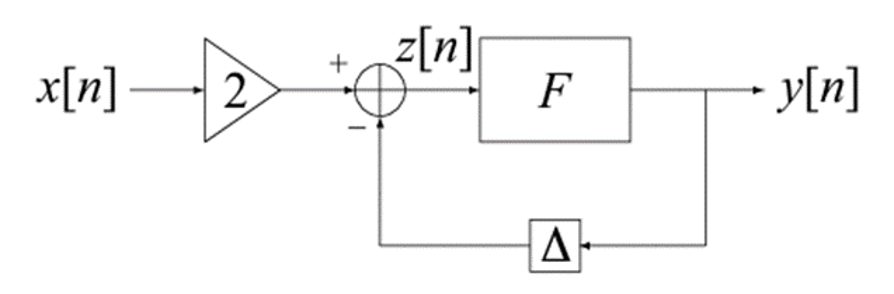
\includegraphics[width=0.7\textwidth]{images/image1}
    \end{center}
    \noindent The system \( F \) is defined by the input-output relationship:
    \[
    F\{z[n]\} = z[n] - z[n-1]
    \]
    
    \noindent and \( \Delta \) is the unit delay operator:
    \[
    \Delta\{\omega[n]\} = \omega[n - 1]
    \]
    
    \noindent \textbf{Derive the linear difference equation describing this system.} \textbf{(5 marks)}
  
    \subsection*{Solution.} Let \( z[n] \) be the output of the summer, as shown above. Then
    \[
    y[n] = F\{z[n]\} = z[n] - z[n-1].
    \]
    
    Now,
    \[
    z[n] = 2x[n] - \Delta\{y[n]\} = 2x[n] - y[n-1].
    \]
    Therefore, substituting the expression for \( z[n] \) into the first equation, we can write
    \[
    \begin{aligned}
    	y[n] &= z[n] - z[n-1] \\
    	&= \underbrace{2x[n] - y[n-1]}_{=z[n]} - \underbrace{2x[n-1] - y[n-2]}_{=z[n-1]} \\
    	&= 2x[n] - y[n-1] - 2x[n-1] + y[n-2].
    \end{aligned}
    \]
    
    \[
    \fbox{y[n] + y[n-1] - y[n-2] = 2x[n] - 2x[n-1]}
    \]
    
    
    
    
    
    \section*{Question 5}
    
    A discrete-time LTI system is described by the following difference equation:
    
    \[
    y(n) = \frac{1}{2}y(n-1) + \frac{3}{8}y(n-2) = x(n) + x(n-1)
    \]
    
    Also, it is given that \( y(-1) = 0 \) and \( x(-2) = -1 \).
    
    \begin{itemize}
    	\item Use the inverse Z-transform to find the \textbf{natural response} of the system.  \textbf{(8 marks)}
    \end{itemize}
    
    \subsection*{Solution – Natural Response of the System}
    
    The natural response is the response of the system due to initial conditions only. Therefore, we set \( x(n) = 0 \). The homogeneous equation becomes:
    
    \[
    y(n) = \frac{1}{2}y(n-1) + \frac{3}{8}y(n-2)
    \]
    
    Rewriting:
    
    \[
    y(n) - \frac{1}{2}y(n-1) - \frac{3}{8}y(n-2) = 0
    \]
    
    Now take the Z-transform of both sides:
    
    \[
    \mathcal{Z}\left\{y(n) - \frac{1}{2}y(n-1) - \frac{3}{8}y(n-2)\right\} = 0
    \]
    
    Using Z-transform properties:
    
    \[
    Y(z) - \frac{1}{2}(z^{-1}Y(z) + y(-1)) - \frac{3}{8}(z^{-2}Y(z) + z^{-1}y(-1) + y(-2)) = 0
    \]
    
    Given: \( y(-1) = 0 \), assume \( y(-2) = A \) (initial condition to be solved for natural response):
    
    \[
    Y(z)\left(1 - \frac{1}{2}z^{-1} - \frac{3}{8}z^{-2}\right) - \frac{3}{8}A = 0
    \]
    
    Solve for \( Y(z) \):
    
    \[
    Y(z) = \frac{\frac{3}{8}A}{1 - \frac{1}{2}z^{-1} - \frac{3}{8}z^{-2}} = \frac{3A}{8} \cdot \frac{z^2}{z^2 - \frac{1}{2}z - \frac{3}{8}}
    \]
    
    Factor the denominator:
    
    \[
    z^2 - \frac{1}{2}z - \frac{3}{8} = \left(z - 1\right)\left(z + \frac{3}{4}\right)
    \]
    
    Thus:
    
    \[
    Y(z) = \frac{3A}{8} \cdot \frac{z^2}{(z - 1)(z + \frac{3}{4})}
    \]
    
    We apply partial fraction decomposition:
    
    \[
    \frac{Y(z)}{z} = \frac{3A}{8} \cdot \frac{z}{(z - 1)(z + \frac{3}{4})} = \frac{B}{z - 1} + \frac{C}{z + \frac{3}{4}}
    \]
    
    Solving for \( B \) and \( C \):
    
    \[
    \frac{z}{(z - 1)(z + \frac{3}{4})} = \frac{B}{z - 1} + \frac{C}{z + \frac{3}{4}}
    \Rightarrow z = B\left(z + \frac{3}{4}\right) + C\left(z - 1\right)
    \]
    
    Let’s solve using substitution:
    
    - Let \( z = 1 \Rightarrow 1 = B\left(1 + \frac{3}{4}\right) \Rightarrow B = \frac{4}{7} \)
    - Let \( z = -\frac{3}{4} \Rightarrow -\frac{3}{4} = C\left(-\frac{3}{4} - 1\right) \Rightarrow C = \frac{3}{7} \)
    
    So:
    
    \[
    \frac{Y(z)}{z} = \frac{3A}{8} \left( \frac{4}{7(z - 1)} + \frac{3}{7(z + \frac{3}{4})} \right)
    \Rightarrow Y(z) = \frac{3A}{8} \left( \frac{4z}{7(z - 1)} + \frac{3z}{7(z + \frac{3}{4})} \right)
    \]
    
    Now take the inverse Z-transform:
    
    \[
    y(n) = \frac{3A}{8} \left[ \frac{4}{7}(1)^n + \frac{3}{7}\left(-\frac{3}{4}\right)^n \right] u(n)
    = \frac{3A}{8} \left[ \frac{4}{7} + \frac{3}{7}\left(-\frac{3}{4}\right)^n \right] u(n)
    \]
    
    \bigskip
    
    \noindent This is the \textbf{natural response} of the system, dependent on the initial condition \( y(-2) = A \). If further information is given about \( y(-2) \), we can substitute it to get the final expression.
   	

    





	\newpage
	\bigskip
	\begin{center}
		\textbf{\LARGE Exam Questions}
	\end{center}
	
	\bigskip
	
	\section*{Exam Question 3(a)}
	
	Consider a sinusoidal signal:  
	\[
	x(t) = 3 \cos(1000\pi t + 0.1\pi)
	\]  
	and let us sample it at a frequency \( F_s = 2 \, \text{kHz} \).
	
	\begin{enumerate}
		\item[(a)] Determine an expression for the sampled sequence \( x[n] = x(nT_s) \) and determine its Discrete Time Fourier Transform \( X(\omega) = \text{DTFT}\{x[n]\} \).
		\item[(b)] Determine \( X(F) = \text{FT}\{x(t)\} \).
		\item[(c)] Recompute \( X(\omega) \) from \( X(F) \) and verify that you obtain the same expression as in part (a).  \textbf{(12 marks)}
	\end{enumerate}
	
	\subsection*{Solution}
	
	\subsection*{(a) Sampled Signal and DTFT}
	
	Sampling with \( T_s = \frac{1}{F_s} = \frac{1}{2000} \), we have:  
	\[
	x[n] = x(nT_s) = 3 \cos(1000\pi n T_s + 0.1\pi) = 3 \cos(0.5\pi n + 0.1\pi)
	\]
	
	Using Euler’s formula:
	\[
	x[n] = 1.5 e^{j0.1\pi} e^{j0.5\pi n} + 1.5 e^{-j0.1\pi} e^{-j0.5\pi n}
	\]
	
	Taking the DTFT:
	\[
	X(\omega) = \text{DTFT}\{x[n]\} = 3\pi e^{j0.1\pi} \delta\left(\omega - \frac{\pi}{2}\right) + 3\pi e^{-j0.1\pi} \delta\left(\omega + \frac{\pi}{2}\right)
	\]
	
	\subsection*{(b) Continuous-Time Fourier Transform}
	
	Since \( x(t) = 3 \cos(1000\pi t + 0.1\pi) \), it can be written as:
	\[
	x(t) = 1.5 e^{j(1000\pi t + 0.1\pi)} + 1.5 e^{-j(1000\pi t + 0.1\pi)}
	\]
	
	Using the Fourier transform property:
	\[
	\mathcal{F}\{e^{j2\pi F_0 t}\} = \delta(F - F_0)
	\]
	
	We get:
	\[
	X(F) = 1.5 e^{j0.1\pi} \delta(F - 500) + 1.5 e^{-j0.1\pi} \delta(F + 500)
	\]
	
	\subsection*{(c) Recomputing \( X(\omega) \) from \( X(F) \)}
	
	Recall the relationship between DTFT and FT:
	\[
	X(\omega) = F_s \sum_{k=-\infty}^{\infty} X(F - kF_s) \bigg|_{F = \frac{\omega F_s}{2\pi}}
	\]
	
	Since there is no aliasing (i.e., the signal is bandlimited to less than \( \frac{F_s}{2} = 1\,\text{kHz} \)), we simplify:
	\[
	X(\omega) = F_s \cdot X(F) \bigg|_{F = \frac{\omega F_s}{2\pi}} = 2000 \cdot X\left(\frac{2000 \omega}{2\pi}\right)
	\]
	
	Substituting \( X(F) \) from part (b):
	
	\[
	X(\omega) = 2000 \left[1.5 e^{j0.1\pi} \delta\left(\frac{2000 \omega}{2\pi} - 500\right) + 1.5 e^{-j0.1\pi} \delta\left(\frac{2000 \omega}{2\pi} + 500\right)\right]
	\]
	
	Using the scaling property of delta functions:
	\[
	\delta(a\omega) = \frac{1}{|a|} \delta(\omega)
	\]
	
	Then:
	\[
	X(\omega) = 3\pi e^{j0.1\pi} \delta\left(\omega - \frac{\pi}{2}\right) + 3\pi e^{-j0.1\pi} \delta\left(\omega + \frac{\pi}{2}\right)
	\]
	
	\noindent This matches the result from part (a), verifying the consistency of the transform pair.
	
	
	
	
	\section*{Exam Question 3(b)}
	
	Let \( y[n] \) denote the convolution of \( h[n] \) and \( g[n] \), where
	\(h[n] = \left(\frac{1}{2}\right)^n u[n]  \)

	is a causal sequence. If \( y[0] = 1 \) and \( y[1] = \frac{1}{2} \), find the value of \( g[1] \).  \textbf{(8 marks)}
	
	\subsection*{Convolution sum is defined as:}
	\[
	y[n] = h[n] * g[n] = \sum_{k=-\infty}^{\infty} h[k] g[n-k]
	\]
	
	\subsection*{For a causal sequence}
	\[
	y[n] = h[0] g[n] + h[1] g[n-1] + h[2] g[n-2] + \ldots
	\]
	
	\textbf{For \( n = 0 \):}
	\[
	y[0] = h[0] g[0] + h[1] g[-1] + \ldots
	\]
	Since \( h[n] \) is causal, \( h[n] = 0 \) for \( n < 0 \), and similarly for \( g[n] \). So:
	\[
	y[0] = h[0] g[0]
	\]
	
	\textbf{For \( n = 1 \):}
	\[
	y[1] = h[0] g[1] + h[1] g[0] + h[2] g[-1] + \ldots
	\]
	\[
	y[1] = h[0] g[1] + h[1] g[0]
	\]
	
	Given:
	\[
	h[0] = 1, \quad h[1] = \frac{1}{2}
	\]
	
	\[
	y[1] = g[1] + \frac{1}{2} g[0]
	\]
	
	Now using the given values:
	\[
	y[0] = h[0] g[0] = 1 \Rightarrow g[0] = \frac{y[0]}{h[0]} = \frac{1}{1} = 1
	\]
	
	Substitute \( g[0] = 1 \) into the equation for \( y[1] \):
	\[
	\frac{1}{2} = g[1] + \frac{1}{2}(1) \Rightarrow g[1] = \frac{1}{2} - \frac{1}{2} = 0
	\]
	
	\subsection*{Final Answer:}
	\[
	g[1] = 0
	\]
	
	\subsection*{Alternative method}
	\[
	y[n] = h[n] * g[n]
	= \sum_{k=-\infty}^{\infty} h[k] \cdot g[n - k]
	\]
	
	\[
	y[0] = \sum_{k=-\infty}^{\infty} h[k] \cdot g[-k]
	= \sum_{k=-\infty}^{\infty} \left(\frac{1}{2}\right)^k U[k] \cdot g[-k]
	= \sum_{k=0}^{\infty} \left(\frac{1}{2}\right)^k g[-k]
	\]
	
	\[
	= g(0) + g(-1) \cdot \left(\frac{1}{2}\right) + g(-2) \cdot \left(\frac{1}{2}\right)^2 + \cdots = 1 \tag{A}
	\]
	
	\[
	y[1] = \left(\frac{1}{2}\right)^0 g[1] + \left(\frac{1}{2}\right)^1 g(0) + \left(\frac{1}{2}\right)^2 g[-1] + \cdots \tag{B}
	\]
	
	\vspace{1em}
	
	\noindent
	Eq$^{n}$ (B) $-$ Eq$^{n}$ (A) $\times \left(\frac{1}{2}\right)$ gives, \\
	\[
	\Rightarrow \frac{1}{2} g[1] = 0
	\Rightarrow g[1] = 0
	\]
	
	
	\section*{Question 4(a)}
	
	A discrete-time LTI system is described by the following difference equation:
	
	\[
	y(n) = \frac{3}{4}y(n-1) - \frac{1}{8}y(n-2) + x(n) + x(n-1)
	\]
	
	Also, it is given that \( y(-1) = 0 \) and \( x(-2) = -1 \).
	
	\begin{itemize}
		\item Use the inverse Z-transform to find the \textbf{natural response} of the system. \textbf{(10 marks)}
	\end{itemize}
	
	\subsection*{Solution – Natural Response of the System}
	
	The natural response is the response of the system due to initial conditions only. Therefore, we set \( x(n) = 0 \). The homogeneous equation becomes:
	
	\[
	y(n) = \frac{3}{4}y(n-1) - \frac{1}{8}y(n-2)
	\]
	
	Rewriting:
	
	\[
	y(n) - \frac{3}{4}y(n-1) + \frac{1}{8}y(n-2) = 0
	\]
	
	Now take the Z-transform of both sides:
	
	\[
	\mathcal{Z}\left\{y(n) - \frac{3}{4}y(n-1) + \frac{1}{8}y(n-2)\right\} = 0
	\]
	
	Using Z-transform properties:
	
	\[
	Y(z) - \frac{3}{4}(z^{-1}Y(z) + y(-1)) + \frac{1}{8}(z^{-2}Y(z) + z^{-1}y(-1) + y(-2)) = 0
	\]
	
	Given: \( y(-1) = 0 \), let \( y(-2) = A \) (unknown initial condition):
	
	\[
	Y(z)\left(1 - \frac{3}{4}z^{-1} + \frac{1}{8}z^{-2}\right) + \frac{1}{8}A = 0
	\]
	
	Solving for \( Y(z) \):
	
	\[
	Y(z) = -\frac{\frac{1}{8}A}{1 - \frac{3}{4}z^{-1} + \frac{1}{8}z^{-2}} = -\frac{A}{8} \cdot \frac{z^2}{z^2 - \frac{3}{4}z + \frac{1}{8}}
	\]
	
	Factor the denominator:
	
	Use the quadratic formula:
	
	\[
	z = \frac{\frac{3}{4} \pm \sqrt{\left(\frac{3}{4}\right)^2 - 4\cdot\frac{1}{8}}}{2}
	= \frac{\frac{3}{4} \pm \sqrt{\frac{9}{16} - \frac{1}{2}}}{2}
	= \frac{\frac{3}{4} \pm \sqrt{\frac{1}{16}}}{2}
	= \frac{\frac{3}{4} \pm \frac{1}{4}}{2}
	\]
	
	So the roots are \( z = \frac{1}{2}, \frac{1}{4} \), hence:
	
	\[
	Y(z) = -\frac{A}{8} \cdot \frac{z^2}{(z - \frac{1}{2})(z - \frac{1}{4})}
	\]
	
	Now apply partial fraction decomposition:
	
	\[
	\frac{Y(z)}{z} = -\frac{A}{8} \cdot \frac{z}{(z - \frac{1}{2})(z - \frac{1}{4})}
	= \frac{B}{z - \frac{1}{2}} + \frac{C}{z - \frac{1}{4}}
	\]
	
	To find \( B \) and \( C \), write:
	
	\[
	z = B\left(z - \frac{1}{4}\right) + C\left(z - \frac{1}{2}\right)
	\]
	
	Substitute:
	- \( z = \frac{1}{2} \Rightarrow \frac{1}{2} = B\left(\frac{1}{2} - \frac{1}{4}\right) \Rightarrow B = 2 \)
	- \( z = \frac{1}{4} \Rightarrow \frac{1}{4} = C\left(\frac{1}{4} - \frac{1}{2}\right) \Rightarrow C = -1 \)
	
	So:
	
	\[
	\frac{Y(z)}{z} = -\frac{A}{8} \left( \frac{2}{z - \frac{1}{2}} - \frac{1}{z - \frac{1}{4}} \right)
	\Rightarrow Y(z) = -\frac{A}{8} \left( \frac{2z}{z - \frac{1}{2}} - \frac{z}{z - \frac{1}{4}} \right)
	\]
	
	Now take the inverse Z-transform:
	
	\[
	y(n) = -\frac{A}{8} \left[ 2\left(\frac{1}{2}\right)^n - \left(\frac{1}{4}\right)^n \right] u(n)
	\]
	
	\[
	\boxed{
		y(n) = \frac{A}{8} \left[ \left(\frac{1}{4}\right)^n - 2\left(\frac{1}{2}\right)^n \right] u(n)
	}
	\]
	
	\bigskip
	
	\noindent This is the \textbf{natural response} of the system, expressed in terms of the unknown initial condition \( y(-2) = A \). If \( A \) is known, you can substitute to get the exact numerical response.
	
	
	
	
	

	
	
\end{document}
